
\documentclass[11pt]{article} % use larger type; default would be 10pt

\usepackage[utf8]{inputenc} % set input encoding (not needed with XeLaTeX)
%%% Examples of Article customizations
% These packages are optional, depending whether you want the features they provide.
% See the LaTeX Companion or other references for full information.

%%% PAGE DIMENSIONS
\usepackage{fancyvrb}
\usepackage{geometry} % to change the page dimensions
\geometry{letterpaper} % or letterpaper (US) or a5paper or....
% \geometry{margin=2in} % for example, change the margins to 2 inches all round
% \geometry{landscape} % set up the page for landscape
%   read geometry.pdf for detailed page layout information

\usepackage{graphicx} % support the \includegraphics command and options
\usepackage{latexsym,amsmath,color}
\usepackage{amssymb}
\usepackage{multicol}

% \usepackage[parfill]{parskip} % Activate to begin paragraphs with an empty line rather than an indent

%%% PACKAGES
\usepackage{booktabs} % for much better looking tables
\usepackage{array} % for better arrays (eg matrices) in maths
\usepackage{paralist} % very flexible & customisable lists (eg. enumerate/itemize, etc.)
\usepackage{verbatim} % adds environment for commenting out blocks of text & for better verbatim
\usepackage{subfig} % make it possible to include more than one captioned figure/table in a single float
% These packages are all incorporated in the memoir class to one degree or another...

%%% HEADERS & FOOTERS
\usepackage{fancyhdr} % This should be set AFTER setting up the page geometry
\pagestyle{fancy} % options: empty , plain , fancy
\renewcommand{\headrulewidth}{0pt} % customise the layout...
\lhead{}\chead{}\rhead{}
\lfoot{}\cfoot{\thepage}\rfoot{}

%%% SECTION TITLE APPEARANCE
\usepackage{sectsty}
\allsectionsfont{\sffamily\mdseries\upshape} % (See the fntguide.pdf for font help)
% (This matches ConTeXt defaults)

%%% ToC (table of contents) APPEARANCE
\usepackage[nottoc,notlof,notlot]{tocbibind} % Put the bibliography in the ToC
\usepackage[titles,subfigure]{tocloft} % Alter the style of the Table of Contents
\renewcommand{\cftsecfont}{\rmfamily\mdseries\upshape}
\renewcommand{\cftsecpagefont}{\rmfamily\mdseries\upshape} % No bold!

\setlength\textheight{9.0in}
\addtolength{\oddsidemargin}{-.875in}
\addtolength{\evensidemargin}{-.875in}
\addtolength{\textwidth}{1.75in}

%%% END Article customizations

%%% The "real" document content comes below...

\title{Brief Article}
\author{The Author}
%\date{} % Activate to display a given date or no date (if empty),
         % otherwise the current date is printed 
\pagestyle{empty}

\newcommand{\angleofdangle}{90}

\newcommand{\green}[1]{{\textrm{#1}}}
\newcommand{\blue}[1]{{\textrm{#1}}}

\newcommand{\code}{\text{\textrm{\green{code}}}}
\newcommand{\coder}{\text{\textrm{\green{code}}}_{\text{\textrm{\green{\scriptsize R}}}}}
\newcommand{\codel}{\text{\textrm{\green{code}}}_{\text{\textrm{\green{\scriptsize L}}}}}
\newcommand{\mycomment}[1]{{\itshape // \quad\blue{#1} \/}}


\begin{document}
%\maketitle

\noindent{\large{\bf Name:}}\underline{~~~~~~~~~~~~~~~~~~~~~~~~~~~~~~~~~~~~~~~~~}


\vspace{8ex}

\begin{center}
~~~
{\Large{\bf
\begin{minipage}{4in}
Final Examination
\\
CS4430 Introduction to Compilers
\\
University of Missouri
\\
Spring 2017
\end{minipage}
}}
\end{center}

\vspace{8ex}~~
~~~~~~~~~~~~~~~~~~~~~~~~~~~~~~~~{\Large
\begin{tabular}{|c|c|r|}
\hline
Problem & Points Possible & Points Scored
\\
\hline
1 & 25 & 
\\
\hline
2 & 10 &
\\
\hline
3 & 25 & 
\\
\hline
4 & 10 &
\\
\hline
5 & 10 &
\\
\hline
6 & 5 & 
\\
\hline
7 & 10 &
\\
\hline
8 & 10 &
\\
\hline
\end{tabular}
}

\vfill
\newpage


\begin{enumerate}

\item {\bf (25 total/12.5 each)} Design code translation schemes in the style we used in class for following expressions. For an example of what I mean by ``translation scheme'', see slide 21 of the ``Semantic Analysis 2'' slides.
\begin{itemize}
\item Conditional expressions: {\bf{(e1 ? e2 : e3)}}.
This expression evaluates {\bf e1} and, if it is {\bf 1}, it evaluates {\bf{e2}} and, otherwise, it evaluates {\bf{e3}}.
\vfill

\item Parallel assignment: {\bf (x1,x2,x3) = (e1,e2,e3)}. This expression performs the assignments {\bf x1=e1}, {\bf x2=e2}, and {\bf x3=e3} in succession.
\vfill
\end{itemize}

\newpage

%%%%%%%%%%%%%%%%%%%%%%%%%%%%%%%%%%%%%%%%%%%%%%%%%%%%%%%%%%%%%%%%%%%%%%%
%%%%%%%%%%%%%%%%%%%%%%%%%%%%%%%%%%%%%%%%%%%%%%%%%%%%%%%%%%%%%%%%%%%%%%%
%%%%%%%%%%%%%%%%%%%%%%%%%%%%%%%%%%%%%%%%%%%%%%%%%%%%%%%%%%%%%%%%%%%%%%%
%%%%%%%%%%%%%%%%%%%%%%%%%%%%%%%%%%%%%%%%%%%%%%%%%%%%%%%%%%%%%%%%%%%%%%%
%%%%%%%%%%%%%%%%%%%%%%%%%%%%%%%%%%%%%%%%%%%%%%%%%%%%%%%%%%%%%%%%%%%%%%%
%%%%%%%%%%%%%%%%%%%%%%%%%%%%%%%%%%%%%%%%%%%%%%%%%%%%%%%%%%%%%%%%%%%%%%%
\item {\bf (10 points)} Circle the best answer:

\begin{tabular}{lcl}
\\
\\
 {\bf{a.}} & T or F & Control may enter a basic block at more than one location.
\\
\\
% {\bf{b.}} & T or F & An example of \emph{strength reduction} optimization is replacing \verb+x << 4+ by \verb+x * 16+.
%\\
%\\
 {\bf{b.}} & T or F &
It is possible to implement graph-coloring register allocation in such a way that\\
&& only
one attempt at graph-coloring is needed.
\\
\\
% {\bf{d.}} & T or F &
%Every language recognized by a regular expression can also be recognized by 
%\\
%&&a context-free grammar.
%\\
%\\
 {\bf{c.}} & T or F &
A compiler optimization always improves program performance.
\\
\\
% {\bf{f.}} & T or F &
%Regular expressions are used to define tokens.
%\\
%\\
 {\bf{d.}} & T or F &
Register spilling can always be used to make an interference graph $n$-colorable, for arbitrary $n$.
\end{tabular}
\vspace{2ex}

{\bf{e.}} Define {\em enabling} optimization.


\newpage
%%%%%%%%%%%%%%%%%%%%%%%%%%%%%%%%%%%%%%%%%%%%%%%%%%%%%%%%%%%%%%%%%%%%%%%
%%%%%%%%%%%%%%%%%%%%%%%%%%%%%%%%%%%%%%%%%%%%%%%%%%%%%%%%%%%%%%%%%%%%%%%
%%%%%%%%%%%%%%%%%%%%%%%%%%%%%%%%%%%%%%%%%%%%%%%%%%%%%%%%%%%%%%%%%%%%%%%
%%%%%%%%%%%%%%%%%%%%%%%%%%%%%%%%%%%%%%%%%%%%%%%%%%%%%%%%%%%%%%%%%%%%%%%
%%%%%%%%%%%%%%%%%%%%%%%%%%%%%%%%%%%%%%%%%%%%%%%%%%%%%%%%%%%%%%%%%%%%%%%
%%%%%%%%%%%%%%%%%%%%%%%%%%%%%%%%%%%%%%%%%%%%%%%%%%%%%%%%%%%%%%%%%%%%%%%
\item  {\bf (25 points)}

Here is a list of optimizations, which we discussed in class. We refer to this list in the following questions. Some of these optimizations are slightly different from those we discussed in class, in which case the difference is explained below.
\begin{itemize}
\item Algebraic simplification (AS). This is slightly more general that constant folding in that it can be applied to expressions that are not necessarily constant. E.g., “x + 0” can be algebraically simplified to “x”, although x is not a constant. Note that every constant fold is an algebraic simplification.

\item Common subexpression elimination (CSE). 
Given an expression that occurs more than once within a basic block, CSE stores that expression in a new temporary variable and replaces the expression with the temporary variable; e.g., CSE might replace the left with the right:
\begin{verbatim}
        x <- foo(v * 3);                 t <- v * 3; 
        if (v * 3 < 9) { ... }           x <- foo(t);
                                         if (t < 9) { ... }
\end{verbatim}


\item Constant propagation (CP). Given an assignment of a constant to a variable “x = c” substitutes constant c for variable x wherever possible. Note that this transformation does not eliminate the instruction “x = c”.

\item Dead code elimination (DCE). \emph{Dead code} is code that has no effect on the behavior of a program and, hence, may be safely eliminated. E.g., if \verb+x+ is never read, then the instruction \verb+x <- 9+ may be safely removed.

\item Expression propagation (EP). Given an assignment a$\leftarrow$e, we allow the entire expression e to be substituted for later uses of a, assuming neither a nor any of the temporaries occurring in e are assigned to again before the use. The code resulting from substituting e for a must be “algebraically simplifiable” to three address code. For e = “1 + y”, 
“x$\leftarrow$a + 1” may be transformed to “x$\leftarrow$1 + y + 1” because it may be simplified to “x$\leftarrow$y + 2”, but
“x$\leftarrow$a + z” may not be transformed to “x$\leftarrow$1 + y + z” because this is no longer three address code.
\end{itemize}

\noindent The graph below represents the evolution of a basic block through multiple optimizations. For each stage of the evolution (i.e., 1, 2 or 3) identify the optimizations applied. N.b.,  there may be more than one application per stage.
\vspace{2ex}

\begin{minipage}{1.6in}
\begin{Verbatim}[frame=single,framesep=2mm]
t8     <- j - 1
t9     <- 4 * t8
temp   <- A[t9]
t10    <- j + 1
t11    <- t10 - 1
t12    <- 4 * t11
t13    <- A[t12]
t14    <- j - 1
t15    <- 4 * t14
A[t15] <- t13
t16    <- j + 1
t17    <- t16 - 1
t18    <- 4 * t17
A[t18] <- temp
\end{Verbatim}
\end{minipage}
%
%
%
\begin{minipage}{0.3in}
{\Large$\Rightarrow_1$}
\end{minipage}
%
%
%
\begin{minipage}{1.6in}
\begin{Verbatim}[frame=single,framesep=2mm]
t8     <- j - 1
t9     <- 4 * t8
temp   <- A[t9]
t10    <- j + 1
t11    <- j
t12    <- 4 * j
t13    <- A[t12]
t14    <- j - 1
t15    <- 4 * t14
A[t15] <- t13
t16    <- j + 1
t17    <- j
t18    <- 4 * j
A[t18] <- temp
\end{Verbatim}
\end{minipage}
%
%
%
\begin{minipage}{0.3in}
{\Large$\Rightarrow_2$}
\end{minipage}
%
%
%
\begin{minipage}{1.6in}
\begin{Verbatim}[frame=single,framesep=2mm]
t8     <- j - 1
t9     <- 4 * t8
temp   <- A[t9]
t12    <- 4 * j
t13    <- A[t12]
t14    <- j - 1
t15    <- 4 * t14
A[t15] <- t13
t18    <- 4 * j
A[t18] <- temp
\end{Verbatim}
\end{minipage}
%
%
%
\begin{minipage}{0.3in}
{\Large$\Rightarrow_3$}
\end{minipage}
%
%
%
\begin{minipage}{1.6in}
\begin{Verbatim}[frame=single,framesep=2mm]
t8     <- j - 1
t9     <- 4 * t8
temp   <- A[t9]
t12    <- 4 * j
t13    <- A[t12]
t15    <- 4 * t8
A[t15] <- t13
t18    <- 4 * j
A[t18] <- temp
\end{Verbatim}
\end{minipage}










%\fbox{\(
%\begin{array}{lcl}
%\mathtt{t8} &\la& j-1
%\\
%t9 &\la& 4 * t8
%\\
%temp &\la& A[t9]
%\\
%t10 &\la& j + 1
%\\
%t11 &\la& t10 - 1
%\\
%t12 &\la& 4 * t11
%\\
%t13 &\la&  A[t12]
%\\
%t14 &\la& j-1
%\\
%t15 &\la& 4 * t14
%\\
%A[t15] &\la& t13
%\\
%t16 &\la& j + 1
%\\
%t17 &\la& t16 - 1
%\\
%t18 &\la& 4 * t17
%\\
%A[t18] &\la& temp 
%\end{array}
%\)
%}
%\[~~
%\Rightarrow^{1}
%~~
%\begin{array}{l}
%\end{array}
%\]

\newpage

For stage 1, circle the answer that best describes the optimizations (1 point each):\newline

\hspace{10ex}
\begin{tabular}{lllll}
\begin{minipage}{1in}
AS was used:\vspace{-3.5ex}
\newline
\begin{enumerate}[(a)]
\item 0 times
\item 1 times
\item 2 times
\item 3 times
\item 4 times
\end{enumerate}
\end{minipage}
&
\begin{minipage}{1in}
CSE was used:\vspace{-3.5ex}
\newline
\begin{enumerate}[(a)]
\item 0 times
\item 1 times
\item 2 times
\item 3 times
\item 4 times
\end{enumerate}
\end{minipage}
&
\begin{minipage}{1in}
CP was used:\vspace{-3.5ex}
\newline
\begin{enumerate}[(a)]
\item 0 times
\item 1 times
\item 2 times
\item 3 times
\item 4 times
\end{enumerate}
\end{minipage}
&
\begin{minipage}{1in}
DCE was used:\vspace{-3.5ex}
\newline
\begin{enumerate}[(a)]
\item 0 times
\item 1 times
\item 2 times
\item 3 times
\item 4 times
\end{enumerate}
\end{minipage}
&
\begin{minipage}{1in}
EP was used:\vspace{-3.5ex}
\newline
\begin{enumerate}[(a)]
\item 0 times
\item 1 times
\item 2 times
\item 3 times
\item 4 times
\end{enumerate}
\end{minipage}
\end{tabular}
%\vfill
\vspace{5ex}

For stage 2, circle the answer that best describes the optimizations (1 point each):\newline

\hspace{10ex}
\begin{tabular}{lllll}
\begin{minipage}{1in}
AS was used:\vspace{-3.5ex}
\newline
\begin{enumerate}[(a)]
\item 0 times
\item 1 times
\item 2 times
\item 3 times
\item 4 times
\end{enumerate}
\end{minipage}
&
\begin{minipage}{1in}
CSE was used:\vspace{-3.5ex}
\newline
\begin{enumerate}[(a)]
\item 0 times
\item 1 times
\item 2 times
\item 3 times
\item 4 times
\end{enumerate}
\end{minipage}
&
\begin{minipage}{1in}
CP was used:\vspace{-3.5ex}
\newline
\begin{enumerate}[(a)]
\item 0 times
\item 1 times
\item 2 times
\item 3 times
\item 4 times
\end{enumerate}
\end{minipage}
&
\begin{minipage}{1in}
DCE was used:\vspace{-3.5ex}
\newline
\begin{enumerate}[(a)]
\item 0 times
\item 1 times
\item 2 times
\item 3 times
\item 4 times
\end{enumerate}
\end{minipage}
&
\begin{minipage}{1in}
EP was used:\vspace{-3.5ex}
\newline
\begin{enumerate}[(a)]
\item 0 times
\item 1 times
\item 2 times
\item 3 times
\item 4 times
\end{enumerate}
\end{minipage}
\end{tabular}
%\vfill
\vspace{5ex}

For stage 3, circle the answer that best describes the optimizations (1 point each):\newline

\hspace{10ex}
\begin{tabular}{lllll}
\begin{minipage}{1in}
AS was used:\vspace{-3.5ex}
\newline
\begin{enumerate}[(a)]
\item 0 times
\item 1 times
\item 2 times
\item 3 times
\item 4 times
\end{enumerate}
\end{minipage}
&
\begin{minipage}{1in}
CSE was used:\vspace{-3.5ex}
\newline
\begin{enumerate}[(a)]
\item 0 times
\item 1 times
\item 2 times
\item 3 times
\item 4 times
\end{enumerate}
\end{minipage}
&
\begin{minipage}{1in}
CP was used:\vspace{-3.5ex}
\newline
\begin{enumerate}[(a)]
\item 0 times
\item 1 times
\item 2 times
\item 3 times
\item 4 times
\end{enumerate}
\end{minipage}
&
\begin{minipage}{1in}
DCE was used:\vspace{-3.5ex}
\newline
\begin{enumerate}[(a)]
\item 0 times
\item 1 times
\item 2 times
\item 3 times
\item 4 times
\end{enumerate}
\end{minipage}
&
\begin{minipage}{1in}
EP was used:\vspace{-3.5ex}
\newline
\begin{enumerate}[(a)]
\item 0 times
\item 1 times
\item 2 times
\item 3 times
\item 4 times
\end{enumerate}
\end{minipage}
\end{tabular}


\newpage
%\setlength{\textwidth}{5in}
%\addtolength{\oddsidemargin}{0.875in}
%\addtolength{\evensidemargin}{0.875in}







%%%%%%%%%%%%%%%%%%%%%%%%%%%%%%%%%%%%%%%%%%%%%%%%%%%%%%%%%%%%%%%%%%%%%%%
%%%%%%%%%%%%%%%%%%%%%%%%%%%%%%%%%%%%%%%%%%%%%%%%%%%%%%%%%%%%%%%%%%%%%%%
%%%%%%%%%%%%%%%%%%%%%%%%%%%%%%%%%%%%%%%%%%%%%%%%%%%%%%%%%%%%%%%%%%%%%%%
%%%%%%%%%%%%%%%%%%%%%%%%%%%%%%%%%%%%%%%%%%%%%%%%%%%%%%%%%%%%%%%%%%%%%%%
%%%%%%%%%%%%%%%%%%%%%%%%%%%%%%%%%%%%%%%%%%%%%%%%%%%%%%%%%%%%%%%%%%%%%%%
%%%%%%%%%%%%%%%%%%%%%%%%%%%%%%%%%%%%%%%%%%%%%%%%%%%%%%%%%%%%%%%%%%%%%%%
\item {\bf{(10 points total)}}.

There are five program points, labeled 1-5, in the graph below. Assume that \underline{there are no live 
variables on exit}. 

\begin{center}
\begin{minipage}{4in}
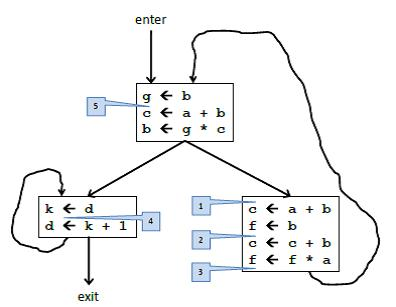
\includegraphics[]{LivenessFigure}
\end{minipage}
\end{center}


\noindent Fill in the following table writing “L” for live and “D” for dead for each program 
point/variable combination.
\newline

~~~~~~~~~~~~~~~~~~
\begin{tabular}{|c|c|c|c|c|c|c|c|c|}
\hline
Program Point & a & b & c & d & e & f & g & k
\\ \hline
1 &~~~~~~&~~~~~~&~~~~~~&~~~~~~&~~~~~~&~~~~~~&~~~~~~&~~~~~~
\\ \hline
2 &&&&&&&&
\\ \hline
3 &&&&&&&&
\\ \hline
4 &&&&&&&&
\\ \hline
5 &&&&&&&&
\\
\hline
\end{tabular}

%%%%%%%%%%%%%%%%%%%%%%%%%%%%%%%%%%%%%%%%%%%%%
%%%%%%%%%%%%%%%%%%%%%%%%%%%%%%%%%%%%%%%%%%%%%
%%%%%%%%%%%%%%%%%%%%%%%%%%%%%%%%%%%%%%%%%%%%%
%%%%%%%%%%%%%%%%%%%%%%%%%%%%%%%%%%%%%%%%%%%%%
%%%%%%%%%%%%%%%%%%%%%%%%%%%%%%%%%%%%%%%%%%%%%
\newpage


%%%%%%%%%%%%%%%%%%%%%%%%%%%%%%%%%%%%%%%%%%%%%%%%%%%%%%%%%%%%%%%%%%%%%%%
%%%%%%%%%%%%%%%%%%%%%%%%%%%%%%%%%%%%%%%%%%%%%%%%%%%%%%%%%%%%%%%%%%%%%%%
%%%%%%%%%%%%%%%%%%%%%%%%%%%%%%%%%%%%%%%%%%%%%%%%%%%%%%%%%%%%%%%%%%%%%%%
%%%%%%%%%%%%%%%%%%%%%%%%%%%%%%%%%%%%%%%%%%%%%%%%%%%%%%%%%%%%%%%%%%%%%%%
%%%%%%%%%%%%%%%%%%%%%%%%%%%%%%%%%%%%%%%%%%%%%%%%%%%%%%%%%%%%%%%%%%%%%%%
%%%%%%%%%%%%%%%%%%%%%%%%%%%%%%%%%%%%%%%%%%%%%%%%%%%%%%%%%%%%%%%%%%%%%%%
\item {\bf (10 points)}
Consider the following control flow graph.
A node $d$ {\underline{dominates}} a node $n$ if every path from the start node to $n$ must go through $d$. By definition, every node dominates itself. The {\underline{dominator set}} of a node is the set of nodes it dominates in the control flow graph.
\begin{center}
~~~~~~~~~~~~~~~~~~~~~~~~~~
\begin{minipage}{4in}
\scalebox{0.5}{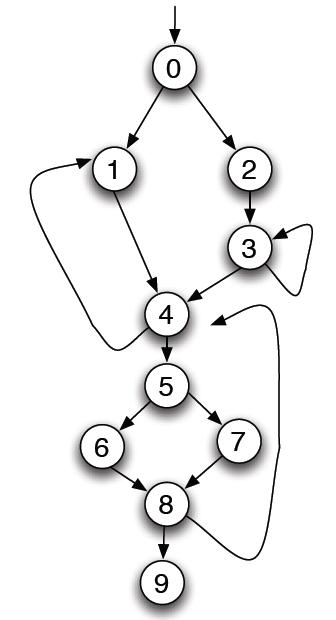
\includegraphics[]{CFG.jpg}}
\end{minipage}
\end{center}

\noindent Fill in the following table.
\newline

~~~~~~~~~~~~~~~~~~
\begin{tabular}{|c|c|}
\hline
Node & Dominator Set 
\\
\hline
0 &~~~~~~~~~~~~~~~~~~~~~~~~~~~~~~~~~~~~~~~~~~~~~~~~~~~~~~~~~~~~~~~~~~~~~~~~~~~~~~~~~~~~~~~~
\\
&\\
\hline
1 &
\\
&\\
\hline
2 &
\\
&\\
\hline
3 &
\\
&\\
\hline
4 &
\\
&\\
\hline
5 &
\\
&\\
\hline
6 &
\\
&\\
\hline
7 &
\\
&\\
\hline
8 &
\\
&\\
\hline
9 &
\\
&\\
\hline
\end{tabular}


\newpage

%%%%%%%%%%%%%%%%%%%%%%%%%%%%%%%%%%%%%%%%%%%%%%%%%%%%%%%%%%%%%%%%%%%%%%%
%%%%%%%%%%%%%%%%%%%%%%%%%%%%%%%%%%%%%%%%%%%%%%%%%%%%%%%%%%%%%%%%%%%%%%%
%%%%%%%%%%%%%%%%%%%%%%%%%%%%%%%%%%%%%%%%%%%%%%%%%%%%%%%%%%%%%%%%%%%%%%%
%%%%%%%%%%%%%%%%%%%%%%%%%%%%%%%%%%%%%%%%%%%%%%%%%%%%%%%%%%%%%%%%%%%%%%%
%%%%%%%%%%%%%%%%%%%%%%%%%%%%%%%%%%%%%%%%%%%%%%%%%%%%%%%%%%%%%%%%%%%%%%%
%%%%%%%%%%%%%%%%%%%%%%%%%%%%%%%%%%%%%%%%%%%%%%%%%%%%%%%%%%%%%%%%%%%%%%%
\item {\bf{(5 points)}}.
If possible, 4-color the following interference graph.
\newline

\begin{center}
\begin{minipage}{6in}
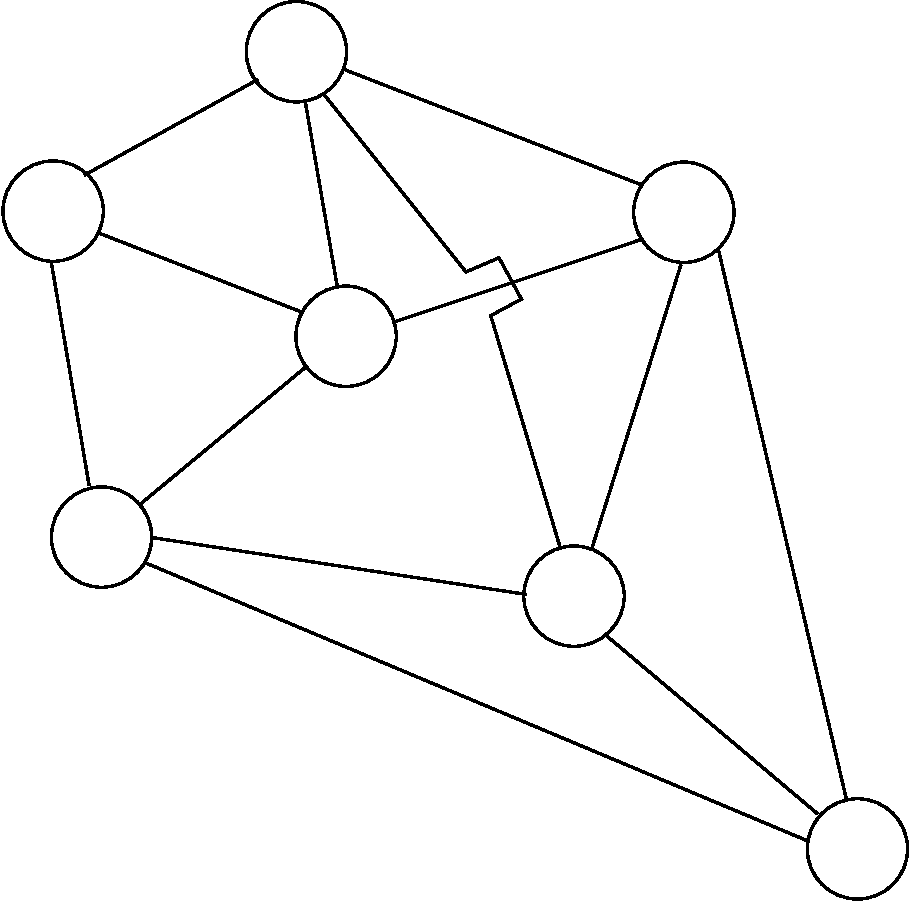
\includegraphics[]{InterferenceGraph}
\end{minipage}
\end{center}



\newpage
%%%%%%%%%%%%%%%%%%%%%%%%%%%%%%%%%%%%%%%%%%%%%%%%%%%%%%%%%%%%%%%%%%%%%%%
%%%%%%%%%%%%%%%%%%%%%%%%%%%%%%%%%%%%%%%%%%%%%%%%%%%%%%%%%%%%%%%%%%%%%%%
%%%%%%%%%%%%%%%%%%%%%%%%%%%%%%%%%%%%%%%%%%%%%%%%%%%%%%%%%%%%%%%%%%%%%%%
%%%%%%%%%%%%%%%%%%%%%%%%%%%%%%%%%%%%%%%%%%%%%%%%%%%%%%%%%%%%%%%%%%%%%%%
%%%%%%%%%%%%%%%%%%%%%%%%%%%%%%%%%%%%%%%%%%%%%%%%%%%%%%%%%%%%%%%%%%%%%%%
%%%%%%%%%%%%%%%%%%%%%%%%%%%%%%%%%%%%%%%%%%%%%%%%%%%%%%%%%%%%%%%%%%%%%%%

\item {\bf{10 points total}}.

Translate the following loop into three-address code.
\begin{verbatim}
                                    for i=j to 2*n step m+k do
                                           s := s+i
\end{verbatim}

\vfill
%%%%%%%%%%%%%%%%%%%%%%%%%%%%%%%%%%%%%%%%%%%%%%%%%%%%%%%%%%%%%%%%%%%%%%%
%%%%%%%%%%%%%%%%%%%%%%%%%%%%%%%%%%%%%%%%%%%%%%%%%%%%%%%%%%%%%%%%%%%%%%%
%%%%%%%%%%%%%%%%%%%%%%%%%%%%%%%%%%%%%%%%%%%%%%%%%%%%%%%%%%%%%%%%%%%%%%%
%%%%%%%%%%%%%%%%%%%%%%%%%%%%%%%%%%%%%%%%%%%%%%%%%%%%%%%%%%%%%%%%%%%%%%%
%%%%%%%%%%%%%%%%%%%%%%%%%%%%%%%%%%%%%%%%%%%%%%%%%%%%%%%%%%%%%%%%%%%%%%%
%%%%%%%%%%%%%%%%%%%%%%%%%%%%%%%%%%%%%%%%%%%%%%%%%%%%%%%%%%%%%%%%%%%%%%%
\item {\bf 10 points total}.

The following is a context-free grammar:
\begin{verbatim}
L -> ident
L -> ( L L )
L -> ( lambda ( ident ) L )
\end{verbatim}

Answer the following questions:
\begin{enumerate}[a.]
\item True or False: the above grammar is ambiguous (\emph{1 point}).

\item  (\emph{1 point}) List the non-terminal symbols.

\item  (\emph{1 point}) List the terminal symbols.

\item (\emph{7 points}) Show a derivation of: \verb+( (lambda(x) x) (u v) )+
\end{enumerate}
\vfill


\end{enumerate}

\end{document}